
\documentclass[11pt]{article}
\usepackage{UF_FRED_paper_style}
\usepackage{xcolor}  % colored text
\usepackage{lipsum}  %% Package to create dummy text (comment or erase before start)
\usepackage{booktabs}  % professional-quality tables
\usepackage{caption}
\usepackage{subcaption}
%\usepackage{emoji}
\usepackage{float}
\usepackage{geometry}


%% ===============================================
%% Setting the line spacing (3 options: only pick one)
% \doublespacing
% \singlespacing
\onehalfspacing
%% ===============================================

\setlength{\droptitle}{-5em} %% Don't touch

% %%%%%%%%%%%%%%%%%%%%%%%%%%%%%%%%%%%%%%%%%%%%%%%%%%%%%%%%%%
% SET THE TITLE
% %%%%%%%%%%%%%%%%%%%%%%%%%%%%%%%%%%%%%%%%%%%%%%%%%%%%%%%%%%

% TITLE:
\title{Kevin Willer IM 2022 Proposal: Sentiment Analysis Domain Transfer}

% AUTHORS:
\author{Kevin Willer\\% Name author
    \href{mailto:kwiller@uni-potsdam.de}{\texttt{kwiller@uni-potsdam.de}} %% Email author 1
    }

% DATE:
\date{\today}

% %%%%%%%%%%%%%%%%%%%%%%%%%%%%%%%%%%%%%%%%%%%%%%%%%%%%%%%%%%
% %%%%%%%%%%%%%%%%%%%%%%%%%%%%%%%%%%%%%%%%%%%%%%%%%%%%%%%%%%
\begin{document}

%{\setstretch{.8}
\maketitle

\section{Problem Introduction}
The proposed research subject in this Individual Research module is based on understandings and realizations gained during previous semester's Project Module on the subject of Sentiment Analysis and Opinion Mining. In the scope of this PM, I set out to (among other goals) adjust a rule-based Sentiment Classifier (\cite{vader}) as to achieve higher classification accuracy on a domain-specific dataset, which the classifier was not prepared for. The domain in this case was that of Tweets concerning Cryptocurrencies. Although I was able to improve the classification accuracy, I identified some shortcomings. The first relates to the obvious flaws that a lexicon-based heuristic model such as VADER brings, such as a lack of context-awareness and semantic understanding. This led me to the idea of applying a BERT-based approach in order to leverage the context-aware embeddings and the attention mechanism (\cite{bert}).
The second shortcoming I identified relates to the syntactic nature of Tweets, which mention, compare or juxtapose multiple entities. Here I seek to apply Aspect-Based Sentiment Analysis (ABSA) (more specifically Aspect Term Sentiment Analysis (ATSA)) in order to achieve a more fine-grained analysis of the sentiment expressed in Tweets.

\section{Theory and Related Work}
With ABSA, one has to differentiate between multiple forms of categorization of aspects. Aspect Category Sentiment Analysis (ACSA) refers to broader, more abstract aspects or categories, which do not necessarily have to be mentioned in the text at all (``It was a cheap and cozy place'', ``cheap'' refering to the category of price, ``cozy'' refering to ambience). Aspect-Term Sentiment Analysis (ATSA) refers to actual entities in the text (``The food was tasty but the neighbourhood was very shady'', ``food'' and ``neighbourhood'' being the entitiy tokens). While the application of ACSA could be interesting in the case of Crypto Twitter data (e.g. finding out which categories of a certain Crypto project are being talked about, be that price action, usability or speed of a Blockchain platform), for this project I am chosing to focus on ATSA, in order to unravel the syntactical structures of the Tweets, when multiple entities are mentioned. \\
I am hereby focussing on the work of \cite{TD-BERT} who successfully modified BERT for use on an ATSA task using different methods of inputting and combining target entity token and text, for every entity in a given text. They use Twitter (\cite{twitter_data}), restaurant and product review (\cite{semeval2016}) data. \\

\section{Procedure and Plan}
The datasets I am planning to focus the research on, which I will apply the models to and evaluate with, is going to be the Crypto-Twitter dataset which I collected in the previous semester using the Twitter API and four Cryptocurrency related queries throughout 2021, many of which are already manually labelled for sentiment and two others consisting of product reviews and Tweets, which were used in the TD-BERT paper and are already preprocessed in a way that the entities are tokenized separately. \\
Since the Twitter dataset which I collected is not yet structured in a way that encodes the information of entities and an exhaustive labelling of the dataset is to time-intensive, I am planning to go for a heuristic approach in order to bootstrap the process of preprocessing, using the API of a Crypto information platform. \\


\begin{figure}[H]
\centering
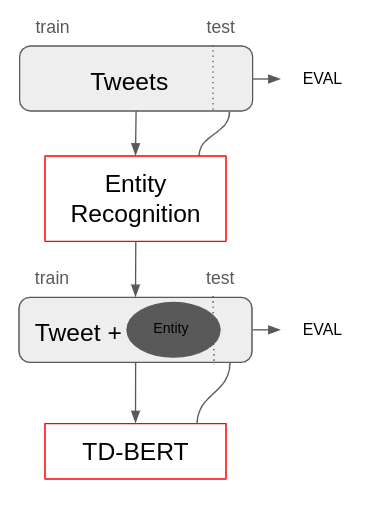
\includegraphics[scale=0.6]{figures/im22_schematic_graph.png}
\caption {Overall schematic graph of project inference and evaluation steps, exemplified by the Cryptocurrency-Twitter dataset. First preprocessing the data so that it is in the shape of ``Text + Entity token'', Second running inference with TD-BERT.}
\label{fig:schema_graph}
\end{figure}

% %%%%%%%%%%%%%%%%%%%%%%%%%%%%%%%%%%%%%%%%%%%%%%%%%%%%%%%%%%
% %%%%%%%%%%%%%%%%%%%%%%%%%%%%%%%%%%%%%%%%%%%%%%%%%%%%%%%%%%
% REFERENCES SECTION
% %%%%%%%%%%%%%%%%%%%%%%%%%%%%%%%%%%%%%%%%%%%%%%%%%%%%%%%%%%
% %%%%%%%%%%%%%%%%%%%%%%%%%%%%%%%%%%%%%%%%%%%%%%%%%%%%%%%%%%
\medskip

\bibliography{references.bib}
\end{document}
